\chapter{基于国产AI处理器的Top-k算子设计实现}
尽管在国产AI处理器架构上已经实现了基于改进的冒泡排序算法的Top-k算子,
但是当数据规模较大的时候,其性能仍然存在一定的不足,并且维护成本相对较高。
因此本文结合国产 AI 处理器的异构计算特点,
根据RadixSelect算法设计了Top-k算子。
具体而言,首先概述了Top-K算法在异构架构下的计算流程。随后,
深入探讨了主机端(CPU)在数据预处理阶段的职责与关键操作。
最后,针对国产 AI 处理器的硬件设计,
详尽阐述了设备端 Top-k 查询算法的实现策略。


\section{国产AI处理器Top-k算子计算流程}
在现代计算领域,伴随大数据的迅猛发展与人工智能技术的持续演进,基于国产AI芯片的Top - k算子计算流程已逐步演化为一种典型的异构计算模式,此模式通常需主机端(如CPU)与设备端(如AI处理器)协同运作。整个计算流程可划分为三个主要阶段:数据准备阶段、数据传输阶段以及核心计算阶段。

1. 数据准备阶段(于主机端执行)
在Top - k算子的整个计算进程中,数据准备阶段起着至关重要的作用,此阶段通常由主机端承担主要职责。在该阶段,主机端(一般为CPU)负责接收输入数据,并对其进行格式转换以及初步的数据清洗操作。鉴于AI处理器往往是针对特定任务进行优化的硬件,其处理能力与CPU存在显著差异,故而需对输入数据进行适配处理,以保障数据能够契合后续硬件计算的要求。

此外,在此阶段,主机端还需对输入数据实施解析与验证操作,旨在确保数据的合法性与有效性。具体工作涵盖检查输入数据的维度、类型等,以保证数据格式与设备端的预期相匹配。在实际应用场景中,此阶段的计算量相对而言较小,然而却是整个计算流程的关键环节,因为若数据准备工作出现偏差,后续计算将无法顺利推进。

2. 数据传输阶段(从主机端向设备端传递数据)
完成数据准备工作后,后续步骤是将经过处理的数据从主机端传输至设备端(AI处理器)。由于AI处理器在处理大规模数据时具备卓越的并行计算优势,此阶段的核心在于将数据高效地传递至设备端,并确保数据在设备端能够进行高效计算。在这一阶段,传输过程的效率直接关乎整体计算性能。倘若数据传输时间过长,将会对整个系统的响应时间产生不利影响。因此,主机端需选取适宜的传输方式,以降低数据传输延迟,确保数据能够尽快抵达设备端。

3. 核心计算阶段(于设备端执行)
核心计算阶段由设备端(AI处理器)负责完成,其主要任务是依据Top - k算子的原理,借助设备端的硬件特性开展高效的并行计算。在传统的CPU环境中,Top - k查询算法通常依赖于单线程或少量线程进行处理,计算效率较低。而在AI处理器中,凭借硬件的向量化计算指令,能够在多个计算单元上并行执行相同操作,从而大幅提升计算速度。故而,设备端的高效计算构成了整个Top - k查询计算流程的核心所在。

通过上述分工,充分发挥了 AI 处理器的硬件优势,显著提高了 Top-k 算法计算效率。在大规模数据处理场景中,该计算流程能够快速筛选出前 k 个最大(或最小)元素,满足数据处理需求。在深度学习领域,可用于模型训练中的数据筛选与特征提取等操作,加速模型训练和推理进程。
图~\ref{fig:topk}展示了本文Top-k算子的计算流程。
\begin{figure}[ht]
    \centering
    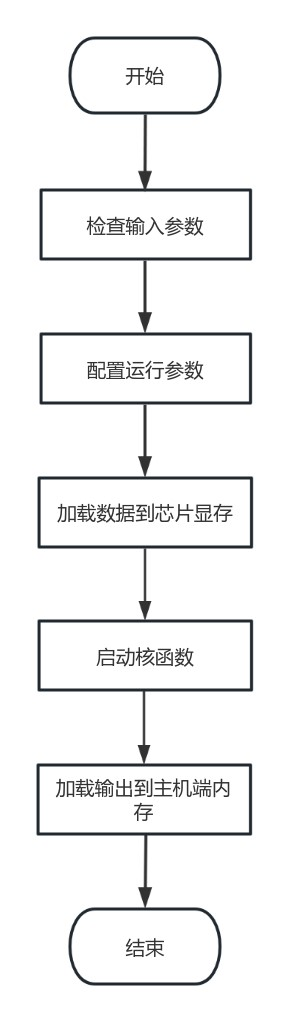
\includegraphics[width=0.3\textwidth]{算子整体流程.jpg}
    \caption{算子整体流程}
    \label{fig:topk}
    % \note{注:图注的内容不宜放到图题中。}
\end{figure}




\section{主机端任务分析}
    \subsection{接口设计及参数检查}
    拟设计实现的 Top-k 算子输入参数要求如表\ref{tab:input_tab}所示,其中,
    keys 表示输入的张量(tensor),其往往含有多个维度。根据所使用的数据类型,
    输入张量的元素值可以为整数或浮点数,
    支持不同的精度(int32 为整数,float32 为浮点数),
    而 values 是挑选出的Top-k元素的下标。dim 表示待操作的维度,k 表示需要得到的前 k 大/小的值。
    假设 keys 数据总共有 n 个维度,并且每个维度的大小为 $\{ x_{0}, x_{1}, \dots, x_{i}, \dots, x_{n-1} \}$,
    则 dim 和 k 所需要满足的数量关系如下:

    \begin{center}
        $0 \leq dim \leq n - 1$
        
        设 dim = i,则: $0 \leq k \leq x_{i}$
    \end{center}
    对于largest,其为bool类型,为true时表示取最大的k个值,为false时,取最小的k个值。
    对于sort,其为bool类型,为true时表示结果需要排序,为false时,不需要将结果进行排序。
    \begin{table}
        \centering
        \caption{输入参数表}
        \label{tab:input_tab}
        \begin{tabular}{cll} % 注意这里是 'cll' 表示三列,第二列和第三列都对齐左侧
          \toprule
          参数名称   & 数据类型                                       & 描述                          \\
          \midrule
          keys & int32/float32 & 输入tensor,可以是任意维度                      \\
          values & int32/uint32 & 输入tensor,可以是任意维度                      \\
          dim & int32   & 表示对第dim维度进行操作            \\
          k   & int32   & 表示取排行前k的数据              \\
          largest & bool   & 默认为true,控制取最大还是最小的值            \\
          sort & bool   & 默认为true,控制是否需要排序            \\
          
          \bottomrule
        \end{tabular}
    \end{table}

    输出参数表如表\ref{tab:output_tab}所示。其中,
    output是最终的输出 tensor,包含通过 Top-k 查询计算得到的Top-k 大/小值。其数据类型可以是 int32 或 float32,具体取决于输入数据的类型以及计算要求。
    output\_values是与 output 对应的下标。它指示从输入数据的第dim维度的哪个位置获取的 Top-k 元素。
    这在需要返回结果的源数据位置时非常有用,尤其是在需要追踪或处理原始数据时。
    \begin{table}
        \centering
        \caption{输出参数表}
        \label{tab:output_tab}
        \begin{tabular}{cll} % 注意这里是 'cll' 表示三列,第二列和第三列都对齐左侧
          \toprule
          参数名称   & 数据类型                                       & 描述                          \\
          \midrule
          output &  int32/float32 & 输出tensor                 \\
          output\_values   & int32/uint32   & 输出数据在排序维度对应的下标              \\
          \bottomrule
        \end{tabular}
    \end{table}

    \subsection{数据处理}
    %数据的预处理和后处理,阐述数据从多维tensor转换为2维tensor
    %以及调用transpose的必要性
    \paragraph{设备端数据摆布方式分析}
    

    Top-k算子需要支持多维度数据,考虑到DLP-M的I/O效率严重受数据在内存中摆放的连续性的影响,因此需要对输入数据进行数据摆放的预处理,以更有效的利用带宽。
    为方便描述,假设其有四个维度,表示如下:\(\text{dim0}\),\(\text{dim1}\),\(\text{dim2}\),
    \(\text{dim3}\)。由左到右表示维度从高到低,按照参数\(\text{dim}\)可以将
    多维度张量(此时为四个维度)转化为三个维度,设其为:
    \(\text{left}\),\(\text{dim}\),\(\text{right}\),其中,\(\text{left}\)为最高维度,
    \(\text{dim}\)为中间维度,
    当\(\text{dim} = 3\)时表示对\(\text{dim3}\)维度进行Top - K查询
    ,此时\(\text{right} = 1\),\(\text{left} = \text{dim0}×\text{dim1}×\text{dim2}\);
    当\(\text{dim} = 0\)时,表示对\(\text{dim0}\)求Top - K,则对应的\(\text{left}\)和
    \(\text{right}\)分别为:\(1\),\(\text{dim1}×\text{dim2}×\text{dim3}\);
    当\(0 < \text{dim} < 3\)时,表示对\(\text{dim}\)求Top - K,则此时left为dim前的维度的乘积,
    right为dim后维度的乘积。

    也就是说,可以将任意维度的数据抽象成一个三维张量,
    其形状为\(\text{left}\),\(\text{dim}\),\(\text{right}\),其中,\(\text{dim}\)是
    待操作维度。但是当\(\text{right}≠1\)时,待
    操作维度不在最低维,这意味进行数据I/O时,将有可能浪费有限的带宽。因此,在
    这种情况下需要针对数据后面两个维度进行转置(transpose)操作,此时张量的形
    状为(\(\text{left}\),\(\text{right}\),\(\text{dim}\)),进一步的
    ,对于Top-k核函数而言,其输入的形状可以抽象为(\(\text{left\_right}\),\(\text{dim}\)),
    其中\(\text{left\_right}=\text{left}×\text{right}\)。当Top - k任务完成之后,输出的形
    状将为(\(\text{left\_right}\),\(\text{k}\)),此时需要对结果再次进行转置操作,其输出形状
    为(\(\text{left}\),\(\text{k}\),\(\text{right}\)),
    作为最终Top - k算子的最终结果。其形状的转变流程如图~\ref{fig:input_shape}
    
    \begin{figure}[ht]
        \centering
        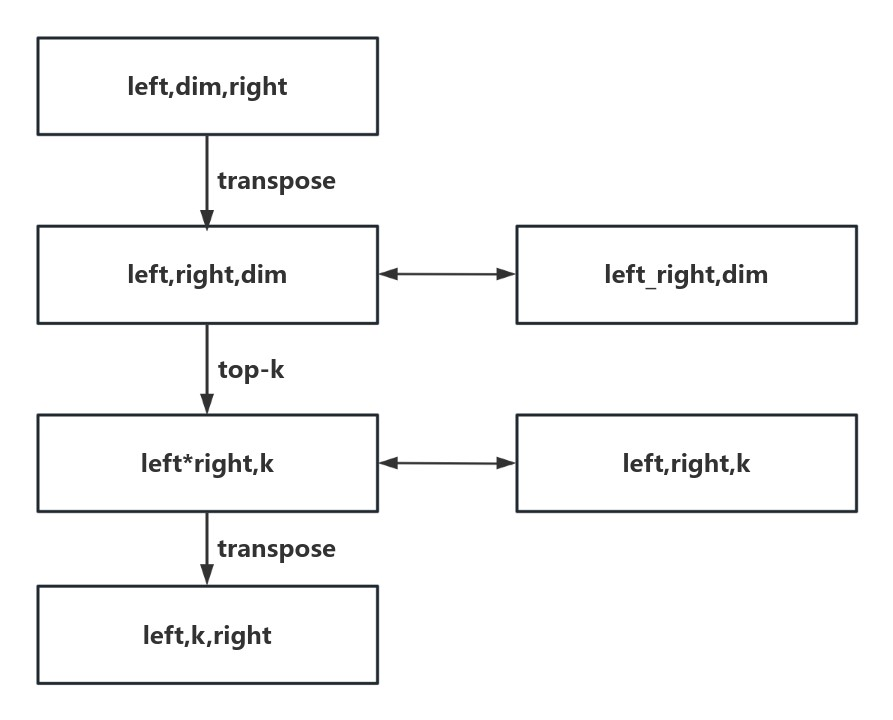
\includegraphics[scale = 0.50]{input_shape.jpg}
        \caption{数据维度变化图}
        \label{fig:input_shape}
        % \note{注:图注的内容不宜放到图题中。}
    \end{figure}
    
    
    \subsection{核函数配置}
    %阐述根据不同规模的输入对kernel函数选取的重要性。
    %阐述各个kernel函数的任务规模配置。
    核函数的配置主要包括三个部分:
    即kernel函数的选取,Job类型的选取和Job数量的确定。
        \paragraph{核函数选取}
        本文基于RadixSelect算法和国产AI处理器的体系结构,实现了两个Top-k核函数,分别处理不同场景下的任务。
        在国产AI处理器的异构计算架构下,根据不同规模的输入合理选取核函数具有至关重要的意义。

        首先,不同规模的输入对系统资源(如内存、计算单元等)的需求不同。在处理大规模输入时,合适的核函数能够合理分配和管理内存资源,确保数据在计算过程中的高效存储和访问。例如,一些针对大规模数据优化的核函数可能采用特定的数据存储格式和访问模式,以减少内存带宽压力,提高数据读取速度,从而充分利用内存资源。同时,在计算单元利用方面,能够根据输入规模动态调整计算单元的使用,避免资源闲置或过度占用。
        对于小规模输入,选择适配的核函数可以避免资源浪费。若使用针对大规模输入设计的核函数处理小规模数据,可能会导致计算单元利用率低下,浪费宝贵的硬件资源。
        另外,在实际应用中,输入规模往往是动态变化的。能够根据不同规模输入灵活选取核函数,使得计算系统具有更好的适应性和可扩展性。无论是面对数据量不断增长的趋势,还是在处理不同规模数据混合的复杂场景中,系统都可以通过选择合适的核函数来应对,从而在不同的应用场景和数据环境下保持良好的性能表现,为系统的长期发展和广泛应用提供坚实基础。




        
        
        \paragraph{Job数量确定}
        对于Job数量而言,这同样涉及到多个方面的重要考量,对于充分发挥国产AI处理器的计算能力和优化程序性能至关重要。
        不同的应用程序具有不同的数据规模和计算复杂度。确定合适的Job数量可以根据具体的计算任务需求,
        将数据和计算负载合理分配到各个Job中。
        对于大规模数据处理任务,可能需要较多的Job来并行处理数据,以加速计算过程;
        而对于相对较小规模的任务,过多的Job可能会导致线程管理开销增加,反而降低性能。因此,根据数据规模和计算需求确定Job数量能够实现计算资源的有效利用,提高计算效率。


        通过前文介绍,我们知道Top-k算子能够处理多维度张量,但是通过一定的数据预处理操作,
        对于Top-k算子的核函数而言,其所需要处理的输入是一个二维张量,并且是在第二个维度提取Top-k个最大/最小元素。
        
        为了方便描述,我们暂且假设问题为:
        设其核函数输入为input,input\_shape = [A, B](在B维度进行操作)。输出为output,output\_shape=[A,k]。

        其中求取最小的Top-k个值。input的数据类型为unsigned\_int(无符号整型)。
        
        我们可以发现,输入数据的每一行之间相互独立,因此我们可以根据行数来确定Job的数量,
        即启动A个Job,每个Job处理一行数据,获取此行数据的k个最小值。Job与数据的对应关系可以通过Job的索引来进行确定。
        因此我们可以将问题进一步聚焦为仅仅只是对于一个长度为B的数组来求取Top-k个最小的值。

        
        \paragraph{Job类型选取}
        在前述内容中提及,国产AI处理器以Task作为最小执行单位,以Job作为最小调度单位,且Job存在多种类型。
        不同的类型通常意味着不同的并行粒度以及Task之间独特的协同方式。

        就Block类型的Job而言,其调度条件相对宽松,仅需一个MLU - Core处于空闲状态即可被调度执行。
        在执行过程中,Job之间不能进行通信,而此时Job仅仅只有一个Task,因此各个Task之间也是逻辑独立的。
        这种独立性体现在MLU-Core执行期间,无需进行通信交互,每个Task能够自主完成自身计算任务而不依赖于其他Task的执行状态或中间结果。
        与之不同的是UnionX任务,其调度要求更为严苛,需要多个MLU - Core同时处于空闲状态方能启动调度。在执行期间,各个Task之间存在复杂的协作关系,具体表现为线程之间需要进行同步操作,以确保任务执行的先后顺序和逻辑正确性。此外,在涉及数据访问时,还需在GDR(全局数据存储)或SMEM(共享内存)上严格维护数据一致性,保证各个Task对数据的读写操作不会产生冲突和错误结果。
        
        因此,Job类型决定了Task的数量,而对于一个Job而言,往往数据规模越大,
        所需要的Task数量往往越多。因此,对于Top-k问题而言,我们可以根据具体实现细节,B的大小和MLU-Core的资源配置情况来确定
        具体的任务类型。
        而这里的资源配置指国产AI处理器的各个层级的内存容量,具体信息如表~\ref{tab:duiqi}所示:


\begin{table}
    \centering
    \caption{内存容量表}
    \label{tab:duiqi}
    \begin{tabular}{cl} % 注意这里是 'cll' 表示三列,第二列和第三列都对齐左侧
      \toprule
      参数名称   & 数据类型        \\
      \midrule
      NRAM / MLU-Core & 512KB     \\
      WRAM / MLU-Core   & 512KB   \\
      SRAM / Cluster& 2MB         \\
      GDRAM       &  80G \\
      \bottomrule
    \end{tabular}
\end{table}
   



\section{设备端并行算法设计与实现}

\subsection{Top-k整体流程设计分析}





基数选择(RadixSelect)是基数排序的一种应用,用于在一组数据中找到具有特定排名的元素。
其算法过程与基数排序算法相似,但与之不同的是,其在迭代的过程中,RadixSelect仅对包含
第 k 大元素的数进行运算,从而达到减少问题规模的效果,另外其输出结果并不是有序的,因此
我们需要对RadixSelect的输出结果根据参数sort来判断是否有必要进行排序。
另外,考虑到国产AI处理器的I/O特点,我们需要根据dim与输入的维度信息关系,
来判断是否有必要对输入/输出进行转置操作。因此,设备端的计算流程如下图~\ref{fig:shebeiliucheng}
所示:

\begin{figure}[ht]
    \centering
    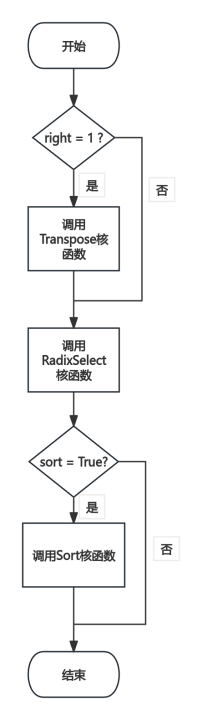
\includegraphics[scale = 0.8]{shebeiliucheng.png}
    \caption{设备端整体流程图}
    \label{fig:shebeiliucheng}
    % \note{注:图注的内容不宜放到图题中。}
\end{figure}


对于Transpose核函数和Sort核函数,可以选用国产AI平台现阶段
已开发好的核函数进行计算;对于RadixSelect核函数,
其主要依托上述提到的RadixSelect算法并结合国产AI处理器的体系结构进行并行设计实现。

在RadixSelect算法中,一个数位(digit)对应着一个元素二进制表示中
的一组连续的\(b\)位。该算法从最高有效数位(most significant digit)到最低有效
数位(least significant digit)处理一个元素,每次迭代处理一个数位。
对于一个由\(r\)位组成的元素,需要进行\(\lceil\frac{r}{b}\rceil\)次迭代
,设为CountingSort,其主要包含四步:
1.求取直方图(HISTOGRAM-KEYS) 
2.扫描桶 (SCAN-BUCKETS) 
3.找到目标桶(FIND-TARGET-BUCKET) 
4.目标元素筛选(FILTER)
,其伪代码见算法~\ref{alg:Counting}。

\begin{algorithm}
    \SetAlgoNoLine 
    % \SetAlgoLined
    % \LinesNumbered            % 强制显示所有行号
    \KwIn{ 数组$Keys$, 代表值; 数组$Values$,代表下标;\\ 
           数组$D$,$Keys$的数位; 整数n,数组长度;
           整数 $k$}
    \KwOut{数组 $Keys\_output$,即最小的k个值;数组 $Values\_output$,即最小k个值的下标;
    $k\_new$ 下轮次的k值
    }
    $Bucket \leftarrow$ init $0$ \tcp{Initialize buckets}
    \tcp{\underline{HISTOGRAM - KEYS}\; }
    \For{$j \leftarrow 0$ to $N - 1$}{
        $Bucket[D[j]] \leftarrow Bucket[D[j]] + 1$
    }
    \tcp{\underline{SCAN - BUCKETS}\; }
    $Sum \leftarrow 0$\;\\
    \For{$i \leftarrow 0$ to $2^r - 1$}{
        $Val \leftarrow Bucket[i]$; $Bucket[i] \leftarrow Sum$\\
        $Sum \leftarrow Sum + Val$
    }
    \tcp{\underline{FIND TARGET BUCKET}\; }
    \For{$i \leftarrow 0$ to $2^r - 1$}{
        \If{$Bucket[i] \ge k$}{
            $POS \leftarrow Bucket[i]$\; $k_new \leftarrow k - Bucket[i-1]$\\
            \textbf{break}\;
        }
    }
    \tcp{\underline{FILTER}\; }
    $offset \leftarrow 0$\\
    \For{$j \leftarrow 0$ to $N - 1$}{
        \If{$D[j] > POS$}{
            \textbf{continue}\;
        }
        \If{$D[j] == POS$}{
            $Keys[offset] \leftarrow Keys[j]$; $Values[offset] \leftarrow Values[j]$; $offset \leftarrow j + 1$\\
            \textbf{continue}\;
        }
        $A \leftarrow Bucket[D[j]]$; $Keys\_output[A] \leftarrow Keys[j]$\\
        $Values\_output[A] \leftarrow Values[j]$; $Bucket[D[j]] \leftarrow A + 1$
    }
    \caption{CountingSort Algorithm}
\end{algorithm}


基于基数排序(Radix Sort)思想的 RadixSelect 算法,在处理大规模数据时,通过按位分组和并行处理,
能有效减少计算时间。特别是在国产AI处理器等并行计算设备上,RadixSelect 算法可以充分利用设备的并行计算
能力,将数据分配到多个计算单元上同时处理。目前RadixSelect算法实现过程中,应当解决的主要问题为以下两个方面:
\begin{enumerate}
    
    \item{并行方案}:
    Top-k的问题适用场景极为宽泛,不同的输入往往对应着不同的实现。在较大数据规模下,
    对于较大的k值,由于片上内存有限,需要将中间计算结果保存在片外空间上。
    而对于较小的 k 值,可以将Top-k 元素常驻在片上内存中,快速响应后续的比较和更新操作,减少对内存的访问延迟。
    因此,本文根据k值与片上空间的大小关系进行了两种并行方案的设计与实现,具体见3.3.2和3.3.3。

    \item{数据类型和正负性}:
    RadixSelect需要从最高位来获取输入数据的数位(digit),需要数据满足“位数越高,数值大小的权重越高”这一规律。
    然而各个类型数据在计算机内存中的存储形式,并不是按照这一形式进行存放的。
    例如对于整型数据而言,负数的数值越大,其对应的二进制越小。
    因此需要根据不同的数据类型对输入数据进行预处理操作,使其满足算法要求。
    同样的,对于大部分有符号数据类型而言,其在内存中的存储形式同样违反“位数越高,数值大小的权重越高”这一规律。
    因此需要根据不同数据类型的正负数的存储规则对输入数据进行预处理操作。具体分析见3.3.4。

\end{enumerate}

\subsection{小k场景下的RadixSelect的并行设计及实现}
为了方便问题的描述,假设输入为无符号整型数据(unsigned)且求取Top-k小元素。
考虑到此时k值较小,中间结果可完全存放在NRAM空间上。在对更复杂的场景进行分析之前,我们在此场景下,先进行单核版本的RadixSelect算法的设计和实现。
即假设此时单个MLU-Core上的片上内存(Nram空间)可以一次性放下input的一行,即B此时相对较小,Job类型设置为Block即可。
  


  
  \paragraph{单核版本}
  根据前文的分析,对于keys-shape = [A,B],我们可以根据A的大小来确定Job的数量,
  单个Job处理输入的若干行,即每个Job处理A\_split行,若是Job的数量小于A的数量,此时单个Job内可使用循环对A\_split行数据进行依次处理,
  而各个Job负责的数据范围,可以根据TaskIdx,TaskIdy和TaskDim等内置变量进行数据与Job之间的
  映射。由于此场景下Job类型为Block,Job只有一个Task,因此Job与Task之间不存在进一步的数据拆分。
  其针对输入数据的拆分示意图如图~\ref{fig:data_split_lk}所示。
  \begin{figure}[ht]
    \centering
    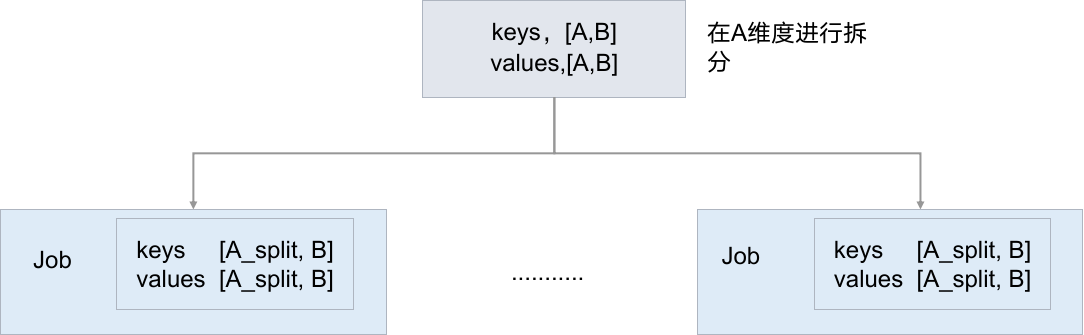
\includegraphics[scale = 0.5]{data_split_lk.png}
    \caption{数据拆分示意图}
    \label{fig:data_split_lk}
    % \note{注:图注的内容不宜放到图题中。}
\end{figure}

我们知道DLP-M具有多级层次存储,且针对不同的层级的存储空间,对于MLU-Core而言其I/O效率和可见性并不一样。在进行数据拆分之后,我们需要进一步设计
各变量的在各存储上的空间划分。结合具体的实现过程,
GDRAM的空间划分如图~\ref{fig:gdr_split_lk}所示。

\begin{figure}[ht]
    \centering
    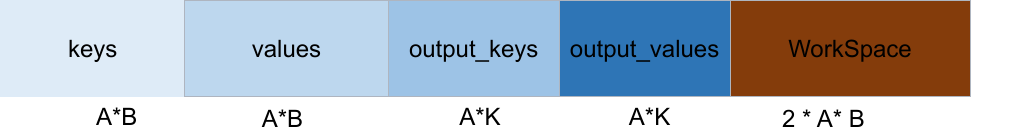
\includegraphics[scale = 0.5]{gdr_split_lk.png}
    \caption{GDRAM空间划分示意图}
    \label{fig:gdr_split_lk}
    % \note{注:图注的内容不宜放到图题中。}
\end{figure}
其中,图中keys所指空间用以存储来自主机端内存的keys数据,values所指空间用以存储来自主机端内存的values数据,
output\_keys和output\_values是最后的输出结果。
workspace所指空间是各Job正常工作时的辅助空间,用以存储辅助变量。
NRAM的空间划分如图~\ref{fig:nram_split_lk}所示。

\begin{figure}[ht]
    \centering
    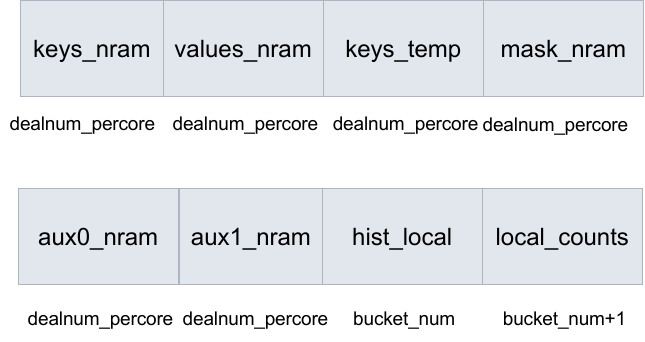
\includegraphics[scale = 0.5]{nram_split_lk.png}
    \caption{NRAM空间划分示意图}
    \label{fig:nram_split_lk}
    % \note{注:图注的内容不宜放到图题中。}
\end{figure}


\begin{table}
    \caption{NRAM空间变量作用说明表}
    \centering
    \begin{tabular}{lcc}
    \toprule
    变量名称 & 长度 & 作用 \\
    \midrule
    keys\_nram & dealnum\_percore & 存储keys \\
    values\_nram & dealnum\_percore & 存储values \\
    keys\_temp & dealnum\_percore & 存储keys当前循环的数位 \\
    aux0\_nram & dealnum\_percore & 存储当前轮次筛选出来的keys \\
    aux1\_nram & dealnum\_percore &  存储当前轮次筛选出来的values\\
    local\_counts & bucket\_num + 1 & 存储前缀和 \\
    hist\_local & bucket\_num & 存储keys的当前digit,落在各个桶中的个数(直方图) \\
    mask\_nram & dealnum\_percore & 掩码向量,表示当前桶中的keys的是否在当前桶中 \\
    \bottomrule
    \end{tabular}
    \label{tab:nram_var}
\end{table}

% 比如,对于GDRAM而言,其对于各个MLU-Core均可见;对于SRAM而言,其对于同一个Cluster内各个MLU-Core均可见,不同Cluster之间不能互相访问;
% 对于NRAM和WRAM而言,是MLU-Core私有存储空间,各个MLU-Core不能互相访问彼此的NRAM和WRAM空间。
\subparagraph{并行实现}
针对核心计算阶段的并行化设计,本文采用多级存储协同与向量化指令优化相结合的策略,具体实现流程如下:

\begin{enumerate}
    \item {初始化}:
    基于 MLU 架构的存储层次特性,首先在 NRAM 空间内执行数据划分策略:根据 MLU-Core 的物理约束条件,为各计算任务分配私有 NRAM 存储区域,并建立对应的数据映射关系。初始化位掩码变量 bit\_mask = 0xF0000000,该参数通过动态右移操作实现迭代过程中数位特征的逐次提取,其偏移量由当前迭代轮次 $t$ 决定,即 bit\_mask $\gg$ 4(t-1)。
    
    \item {构建直方图}:
    采用 bang\_band\_scalar 向量化位操作指令,对 keys\_nram 进行位与运算,提取当前数位特征至 keys\_temp 缓冲。随后通过 bang\_histogram 指令的并行归约能力,统计 keys\_temp 各元素的频率分布,生成局部直方图 hist\_local。此过程通过寄存器级并行实现零拷贝计算,显著降低内存访问延迟。
    
    \item {前缀和计算}:
    基于 bang\_presum 指令的并行扫描特性,对 hist\_local 执行前缀和操作,生成桶边界索引 local\_counts。该指令可在 $O(\log n)$ 时间复杂度内完成全局累积统计,为后续桶选择提供决策依据。
    
    \item {桶搜索}:
    通过线性搜索遍历 local\_counts 数组,求解满足
    \[
    \exists i \in [0,b),\ local\_counts[i] < k \leqslant local\_counts[i+1]
    \]
    的临界桶索引 $i$,并将目标桶键值记录至 key\_bin。该过程引入提前终止机制,当检测到 $k - local\_counts[i] \leqslant \delta$ 时终止搜索($\delta$ 为预设阈值),有效降低分支预测开销。
    
    \item {过滤}:
    \begin{itemize}
    \item 第一级过滤:应用 bang\_le 指令生成掩码 mask\_nram,标记 keys\_temp 中值小于 key\_bin 的位域。通过 bang\_filter 指令配合 mask\_nram,将 keys\_nram 与 values\_nram 的匹配元素存入 aux0\_nram / aux1\_nram,同时使用 bang\_count 统计保留元素数 $k'$,更新 $k \leftarrow k - k'$。
    \item 第二级过滤:采用 bang\_eq 指令定位等于 key\_bin 的元素,通过 bang\_filter 进行选择性保留,并将结果回写至 keys\_nram / values\_nram 作为下一迭代输入。
    \end{itemize}
    \end{enumerate}
    
{优化特性分析}:本实现方案通过(1)NRAM私有化存储消除访存竞争;
(2)向量化指令集提升SIMD效率;
(3)两级过滤降低分支粒度,最终达成计算密度与存储带宽的平衡优化。
实验表明该设计可使Top-K选择算子相较于原版本获得明显的加速比提升,并领先NVIDIA A100 GPU的表现效果。(详见第5章评测部分)。

上述所介绍的算法主要处理中等或较小的数据规模,同时具备处理多维数据的功能,
这使其在网络模型数据处理中尤为有效。然而,该算子并未直接为多核并行处理提供内置逻辑。
对于较大的数据规模,需要配合其他特定算子实施处理策略。具体操作流程包括:在执行Top-k算子
之前,首先应用基于深度学习处理器的 Split 算子,对数据集进行适当划分,
以适配至各个单独的处理核心,期望数据能够被单核心处理。
而后每个核心独立完成指定的 Top-k 计算任务后,应用 Concat 算子将各核返回的数据集成为
最终结果。此步骤完成后,系统可继续执行随后的数据传输与处理操作。这一处
理策略确保了在维持计算效率的同时,能够对大规模数据集进行有效管理和运算。
单核在多核运行环境下的执行顺序如下图\ref{fig:duohe_split}所示。
\begin{figure}[ht]
    \centering
    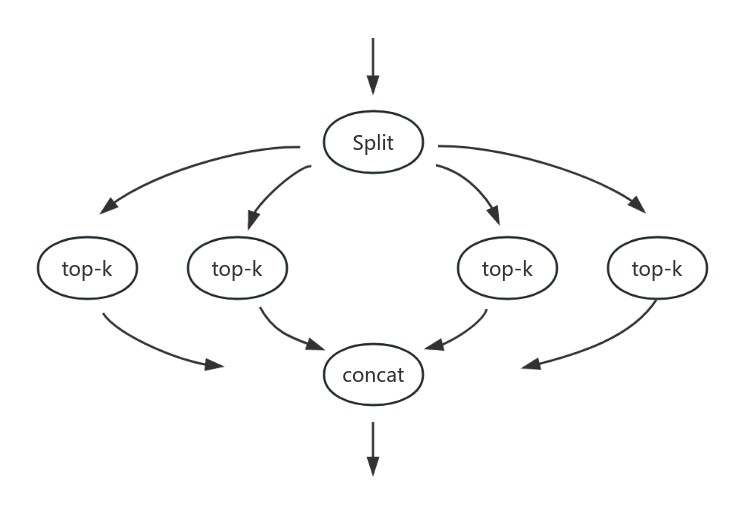
\includegraphics[scale = 0.75]{multicore_data_split.jpg}
    \caption{多核拆分示意图}
    \label{fig:duohe_split}
    % \note{注:图注的内容不宜放到图题中。}
\end{figure}

Split和 Concat 操作是I/O类型算子,也就是说单核 RadixSelect 算法的实现方案在多核上
执行,势必会引入 Split 和 Concat 的额外时间开销,在某些极端的场景下,这可能会成为性能瓶颈。


\paragraph{多核版本}
由于单核RadixSelect的整个操作都是在NRAM空间上进行,需要其输入,输出和各种中间变量的内存容量大小总和
不能超过NRAM的空间大小(即512kb),所以对B的大小要求比较严格(数量级在$10^5$)。
而若是想处理更大规模的数据(B较大时),则需要在深度学习框架侧
调用额外的算子去配合使用。但是这又会增加额外的时间开销,导致算子的整体性能较差。
因此针对小k场景,设计多核RadixSelect是十分必要的。

大规模数据处理方法之一是充分发挥深度学习处理器的多核优势,减轻多核拆分后单核数据处理的负担。首先,依据处理器核心数量\(corenum\),按照数据规模对查询工作
进行划分,从而确定每个核心所需处理的数据量。每个核心对划分后的数据执行Top-k查询,会返
回k个数。多核完成Top-k查
询后,返回的临时数据总量为\(corenum×k×2\)。这里的系数\(2\)是因为包含了返回的\(k\)个数据及其对应的下标。之后,对总量
为\(corenum×k×2\)的数据进行Top-k归并操作。若数据量仍然较大,则再次采用多核Top-k方法处理;若数据
量不大
,则直接用单核Top-k进行归并操作,最终完成整个Top-k查询。需要注意的是,临时数据需要在片外进行缓存,
缓存内容
为每个核心查询返回的Top-k值及其对应的下标。
对应的操作流程可概括为图\ref{fig:multi_core_littlek}所示。
\begin{figure}[ht]
    \centering
    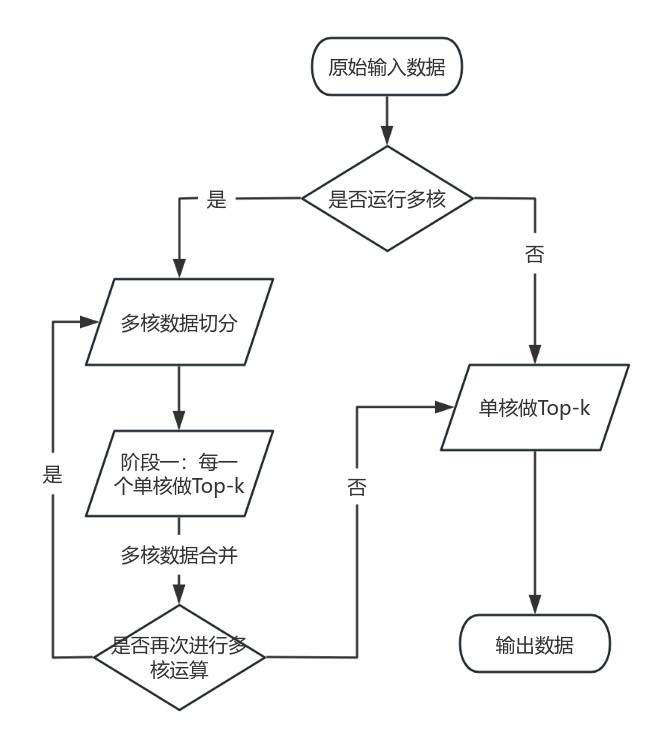
\includegraphics[scale = 0.8]{multi_core_littlek.jpg}
    \caption{Top-k多核实现流程图}
    \label{fig:multi_core_littlek}
    % \note{注:图注的内容不宜放到图题中。}
\end{figure}
    
% 这里依据核心数量和数据量大小进行了精细的区分。当数据量较小时,若采用多核Top-k无法带来好处,那么可考虑使用单核Top-k来执行Top-k查询操作。
% 而当数据量极大时,则要对数据进行多核划分,让每个核心分别完成各自的Top-k查询,之后再依据数据量大小进行下一轮
% Top-k查询。此时所用的多核数量将会更少,如此循环直至完成整个Top-k查询。

% 对于此种方案,多次多核Top-k查询适用于处理大规模的数据情况。
% 例如,在一个具有48个核心的处理器上处理数据量在960万以上且要获取1万Top-k数据的操作时,
% 即便每个核心完成了Top-k筛选,仍会剩余48万的数据需要进一步进行Top-k筛选,数据量依旧庞大。
% 所以,合理地确定好Job类型来进行Top-k筛选至关重要。而对于每一次的多核查询,
% Job的类型决定了核心的数量,设其为Corenum。设单核能够处理的数据数量为num,则

% Corenum = Ceil(( B - 1 ) / num + 1),
% 而UnionX中的X = log(4,Corenum) + 1。

% 但是需要注意的是,由于片上计算空间存在限制,在大规模查询后,需要将
% 计算结果临时存储在片外空间,作为下一次多核/单核查询的输入,这就涉及到片上和片外存储空间频繁的数据交互以及
% 当数据规模超大时多次启动核函数等方面耗费一定的时间。

在核心数量和数据量大小的综合影响下,我们对Top-k查询性能进行了详细分析。对于较小的数据量,如果使用多核Top-k查询并不能带来明显的性能提升,则推荐使用单核Top-k进行查询。相反,对于较大的数据量,应该在多个核心上分配查询任务,使每个核心分别完成自己的Top-k查询,并根据剩余数据量的大小决定是否需要进一步的查询迭代。

例如,在一个拥有48个处理核心的系统中处理超过960万条数据,目标是获取1万个Top-k数据的情形中,尽管每个核心完成了初次Top-k筛选,但总体上仍有大量数据需要进一步处理。因此,每次多核查询后,都需要精确地调整任务类型和核心数量,以确保数据处理的高效性。

具体地,设需要的核心数为\( \text{Corenum} \),单个核心可以处理的数据量为\( \text{num} \),则有:
\[
\text{Corenum} = \left\lceil \frac{B - 1}{\text{num}} + 1 \right\rceil,
\]
其中\( B \)为总数据量。在UnionX结构中的\( X \)值由下式给出,Union0视为Block:

\[
X = 
\begin{cases} 
2^{\lfloor \log_2(\text{Corenum} - 1) \rfloor - 1} & \text{when } \text{Corenum} > 2,\\
1 & \text{when } \text{Corenum} = 2,\\
0 & \text{when } \text{Corenum} = 1.
\end{cases}
\]


值得注意的是,由于硬件的限制,大规模数据查询后,需要将计算结果暂存到外部存储中,为后续的查询过程服务。这种频繁的数据交换和多次核心启动虽然确保了处理大规模数据的能力,但也相应地增加了时间成本。



% 通过上述的分析,可以发现各个MLU-Core之间的Top-k操作相对独立,仅仅是在DDR上汇总Top-k结果时,
% 才需要进行通信,因此针对此核函数,将其Job类型设置为Block类型即可。


  \subsection{大k场景下的RadixSelect的并行设计及实现}
%   国产 AI 处理器具备多核心架构且支持并行运算,在处理维度为\((A,B)\)的输入数据时,算法的并行度显著受制于\(A\)与\(B\)的维度特性。
%   于特定情境下,当\(A\)取值较小(低于\(10\))而\(B\)取值较大(超出\(100\)万)时,单核处理方式会引发严峻的负载均衡困境。具体表现为:其一,凭借\(A\)维度所构建的并行度匮乏,致使部分核心处于闲置状态,无法充分发挥其计算效能;其二,由于\(B\)的规模庞大,被分配任务的核心将持续处于工作负载之下,难以实现高效的资源分配与利用。
%   鉴于上述挑战,本研究精心设计并成功实现了适用于多核处理的 radix - select Top - k 算子。该算子旨在通过多核协同机制,有效缓解因维度不均衡所导致的负载失衡问题,充分挖掘国产 AI 处理器多核心架构的并行计算潜力。
%   此外,参数\(k\)的取值规模与算子的具体实现策略紧密关联。当\(k\)较大(例如超越片上内存 NRAM 的存储容量)时,不可避免地需将临时输出数据暂存于片外空间 GDR。然而,如前文所阐述,GDR 作为存储层级中带宽最低的部分,其数据传输速率严重制约程序的整体性能表现。
%   故而,本研究进一步依据\(k\)的不同取值范围,系统性地设计并实现了具有针对性的 Top - k 算子。
%   后续将对相关设计与实现细节予以详尽阐释。

  前面所介绍的各个实现方案,充分利用了“小k”场景下的一个重要特性——NRAM空间能够存放完整的临时输出。
  而由于NRAM的空间十分有限,因此k的范围不能够太大,否则将会导致程序崩溃。
  因此,针对大k场景下的RadixSelect,必须考虑将临时输出存储在GDR空间上。
  
  回顾RadixSelect的串行算法,由于其所有阶段都存在循环依赖关系,所以不能直接进行并行化(或向量化)。
  例如,如果试图对"构建直方图"(HISTOGRAM - KEYS)的迭代进行并行处理,可能会有多个处理器同时尝试
  对同一个桶(bucket)进行递增操作,产生资源竞争。而如果锁定桶,当有许多键具有相同数位时,
  桶将成为串行瓶颈,将会极大地降低性能。基于以上的分析,可以通过为每个处理器分配一组独立的桶(本地桶),
进而在不需要对桶进行锁定的情况下实现算法并行化:
即每个处理器负责其自己的局部数据(\(\frac{N}{P}\)子集),
并将它们列入自己的本地桶集合中。
此时,可以将所有的桶看作是一个矩阵\(Buckets[i, j]\),
如下图~\ref{fig:process_bucket}所示。

\begin{figure}[ht]
    \centering
    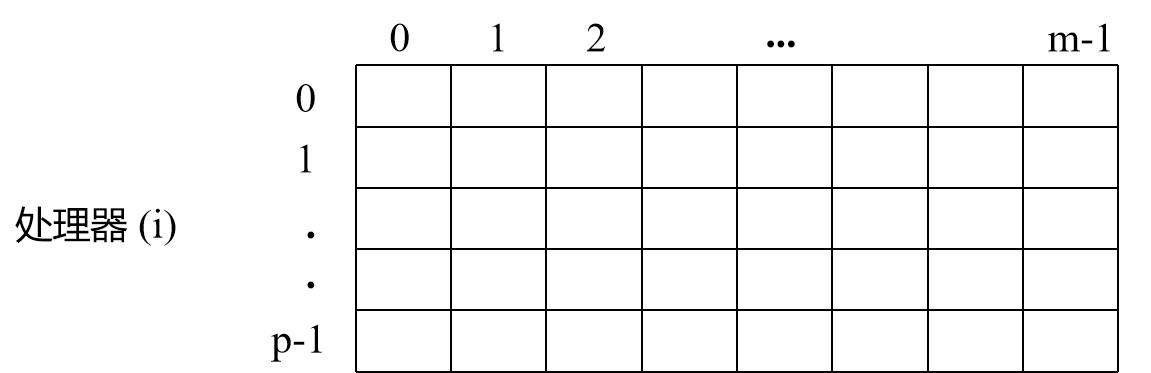
\includegraphics[scale = 0.6]{process_buckets.jpg}
    \caption{处理器组织方式示意图}
    \label{fig:process_bucket}
    % \note{注:图注的内容不宜放到图题中。}
\end{figure}

其中 $i$ 是处理器数,$j$ 是本地桶的桶数。在每个处理器都拥有自己的桶之后,
每个处理器在进行基数选择的
第一阶段,第三阶段和第四阶段(HISTOGRAMKEYS , FIND-TARGET-BUCKET和 FILTER)时,
都在自己的局部数据上进行工作,从而解除所有依赖项。
但需要注意到,为了保证结果的正确性,第三阶段( SCAN-BUCKETS )将必须进行修改。因为如果
每个处理器仅扫描自己的本地桶,将仅仅只能得到局部数据的Top-k结果,导致结果错误。
而通过分析我们发现,
$Buckets[i][j]$代表在进行SCAN-BUCKETS处理后,$A$中元素最终在结果$R$中的偏移位置,
具体关系见下图~\ref{fig:digits}。
\begin{figure}[ht]
    \centering
    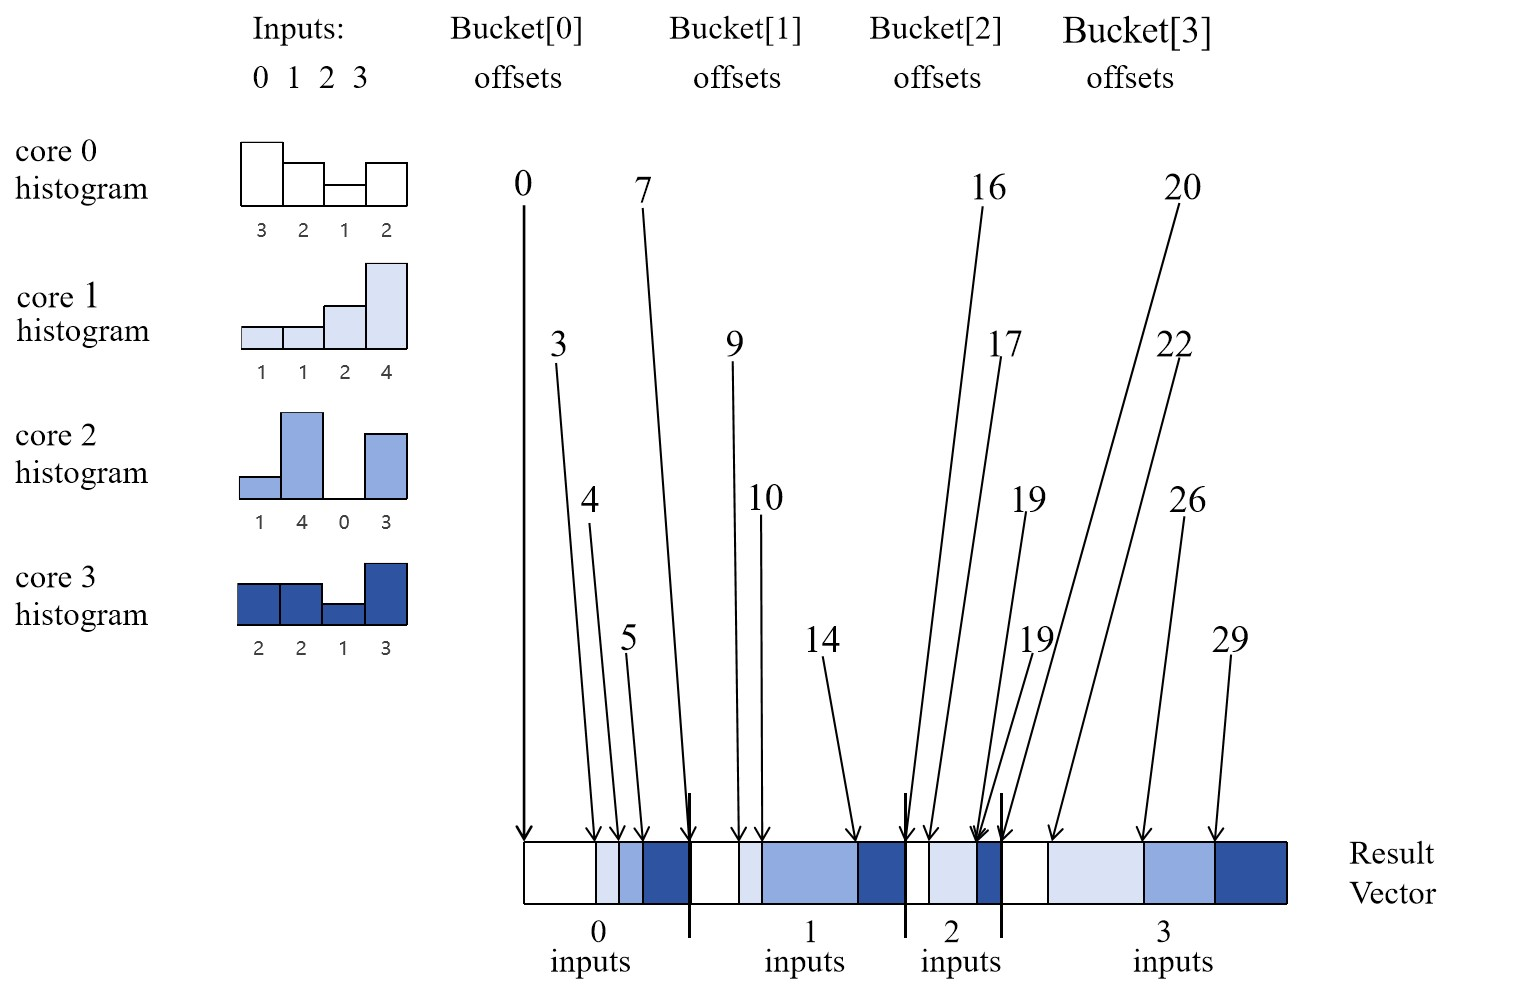
\includegraphics[scale = 0.6]{process_digits.jpg}
    \caption{并行RadixSelect的扫描步骤}
    \label{fig:digits}
    % \note{注:图注的内容不宜放到图题中。}
\end{figure}

假如该算法用 4 个处理器和 4 个桶来对 0 - 3 的值进行排序。偏移量是通过扫描桶来计算的。
扫描之后,每个处理器在具有特定值的键的最终输出中都有一个起始位置。
例如,处理器 3 将把值为 “0” 的键从输出中的第 5 个位置开始放置,把值为 “1” 的键从第 14 个位置开始放置,如偏移量所示。

所以需要将矩阵\(Buckets[i, j]\)在列方向上以及行方向上进行扫描操作,以汇总全局信息,
其数学公式见~\ref{equ:buckets}
\begin{equation}
    \text{ Buckets}[i, j]' = \sum_{k = 0}^{p - 1} \sum_{m = 0}^{j - 1} \text{ Buckets}[k, m] + \sum_{k = 0}^{i - 1} \text{ Buckets}[k, j]
    \label{equ:buckets}
\end{equation}
也就是说,偏移量是所有处理器中小于 $j$ 的数位总数,再加上小于 $i$ 的处理器中数位等于 $j$ 的数量。
这个总和可以通过将$Buckets$矩阵先按列进行求和,然后再对最后一行进行求和,这样,最后一行将存有全局的直方图信息。
而后对此执行前缀和计算,获取全局的前缀和信息。最后将与处理器相同ID的一行,加上全局的前缀信息即可获得当前处理器的前缀和信息,
此前缀信息可以作为FILTER阶段,将结果并行的从NRAM放回GDRAM上的偏移值。
同时,找到目标桶这一阶段,Bucket数组中,仅Buckets的最后一行具有全局的前缀信息,主要对其进行遍历。
上述主要介绍的是针对单行数据,多核数据的并行运算方式。
下面进一步介绍如何将二维数据进行拆分。
已知此时Job类型为UnionX,将会拥有多个Task。因此,我们需要对数据进行二维拆分。
首先,每个Job负责若干行数据,即在A维度进行拆分,共拆分得到
A\_split行数据。对于相同Job中的Task而言,进一步在B维度进行拆分,对于单行数据而言,
一个Task得到的数据为B\_split个数。具体的数据拆分示意图如图~\ref{fig:data_split_bk}所示。

\begin{figure}[ht]
    \centering
    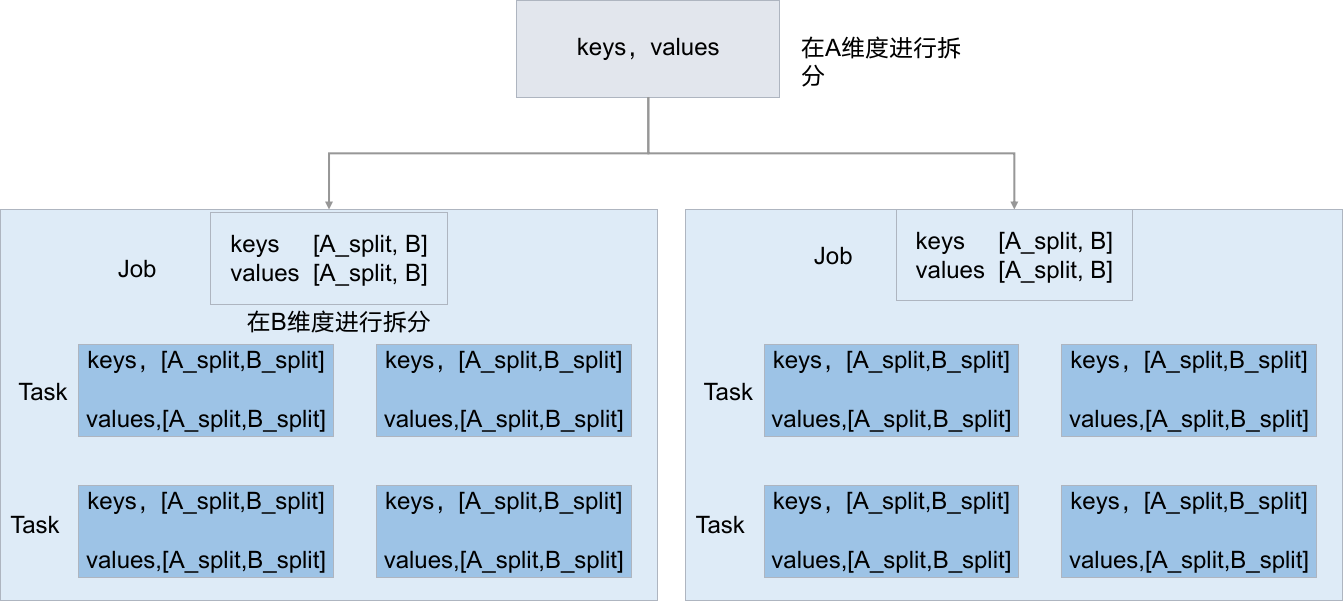
\includegraphics[scale = 0.40]{data_split_bk.png}
    \caption{数据拆分示意图}
    \label{fig:data_split_bk}
    % \note{注:图注的内容不宜放到图题中。}
\end{figure}
当B\_split数据仍然大于NRAM空间时,此时需要将B\_split进一步划分为若干段,
使用循环依次将数据加载到NRAM空间进行处理。
在硬件层面,上述数据拆分过程主要考虑的是各个MLU-Core应该计算哪些输入数据。
而对于具体的实现过程,首先需要考虑输入数据和其他中间变量在各层存储中的空间划分。对于GDRAM而言,主要分为keys,values,output\_keys,
output\_values和Workspace五块区域,各个变量的作用如下表~\ref{tab:gdram_var_bk}所示,
\begin{table}
    \caption{GDRAM空间变量说明表}
    \centering
    \begin{tabular}{lcc}
    \toprule
    变量名称 & 长度 & 作用 \\
    \midrule
    keys & A * B & 存储输入 \\
    values & A * B & 存储下标 \\
    output\_keys & A * B & 存储输出 \\
    output\_values & A * B & 存储输出的下标 \\
    workspace & A * B & 存储中间变量 \\
    \bottomrule
    \end{tabular}
    \label{tab:gdram_var_bk}
\end{table}
其空间划分如图~\ref{fig:gdram_split_bk}所示,
\begin{figure}[ht]
    \centering
    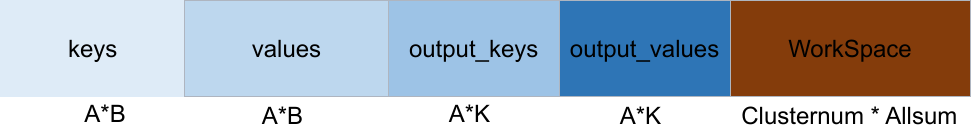
\includegraphics[scale = 0.45]{gdram_split_bk.png}
    \caption{GDRAM空间拆分示意图}
    \label{fig:gdram_split_bk}
    % \note{注:图注的内容不宜放到图题中。}
\end{figure}
值得注意的是,此场景主要针对大规模数据。
此时单个MLU-Core上的NRAM上的空间已经不能够完全放下一行数据,
即单个MLU-Core所负责的数据规模远大于NRAM空间一次能够处理的数据。
此时需要将某些中间结果暂存在GDRAM上,因此将workspace进一步划分为counts\_ddr,batch\_iter\_workspace和values\_batch\_iter\_workspace,
如图~\ref{fig:workspace_split_bk.png}所示。
其中counts\_ddr主要用于存储各个MLU-Core的局部前缀信息,主要达到同步信息的作用。
batch\_iter\_workspace主要存储每次循环执行CountingSort算法时的输入,即筛选之后的输入数据。
values\_batch\_iter\_workspace同理。
\begin{figure}[ht]
    \centering
    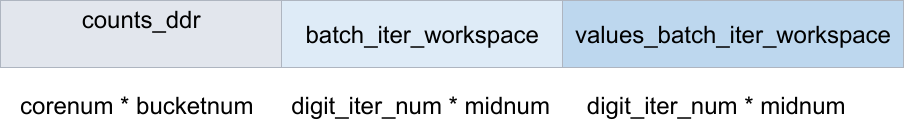
\includegraphics[scale = 0.45]{workspace_split_bk.png}
    \caption{Workspace空间拆分示意图}
    \label{fig:workspace_split_bk}
    % \note{注:图注的内容不宜放到图题中。}
\end{figure}

对于NRAM空间而言,主要涉及的变量及其作用如表~\ref{tab:nram_var_bk}所示,其空间划分如图~\ref{fig:nram_split_bk}所示。
\begin{table}
    \caption{NRAM空间变量说明表}
    \centering
    \begin{tabular}{lcc}
    \toprule
    变量名称 & 长度 & 作用 \\
    \midrule
    keys\_nram & dealnum\_percore & 存储keys \\
    values\_nram & dealnum\_percore & 存储values \\
    keys\_temp & dealnum\_percore & 存储keys当前循环的数位 \\
    aux0\_nram & dealnum\_percore & 存储当前轮次筛选出来的keys \\
    aux1\_nram & dealnum\_percore &  存储当前轮次筛选出来的values\\
    local\_counts & bucket\_num + 1 & 存储全局前缀和 \\
    hist\_global & bucket\_num * (corenum+1) & 用以计算全局的直方图信息 \\
    hist\_local & bucket\_num & \parbox{8cm}{存储当前片段的keys的digit,落在各个桶中的个数(直方图),并且作为offset,将输出并行放置到GDR上} \\
    cur\_hist & bucket\_num & \parbox{8cm}{hist\_local的累加器,用以计算当前Task所负责局部数据的直方图} \\
    mask\_nram & dealnum\_percore & 掩码向量,表示当前桶中的keys的是否在当前桶中 \\
    \bottomrule
    \end{tabular}
    \label{tab:nram_var_bk}
\end{table}

\begin{figure}[ht]
    \centering
    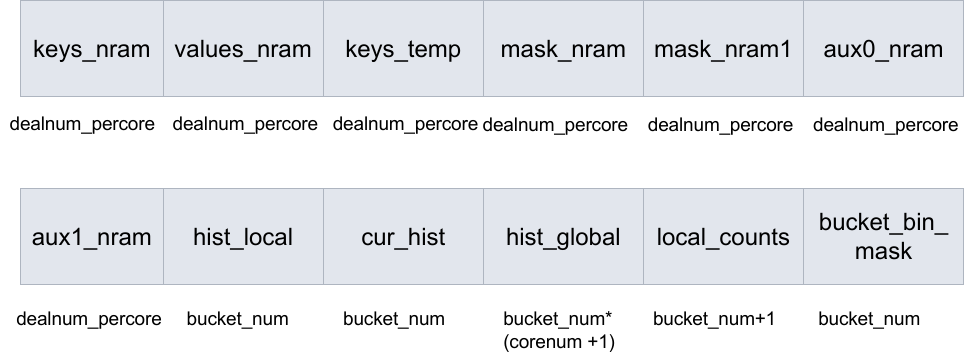
\includegraphics[scale = 0.45]{nram_split_bk.png}
    \caption{数据拆分示意图}
    \label{fig:nram_split_bk}
    % \note{注:图注的内容不宜放到图题中。}
\end{figure}


%Todo


% \begin{enumerate}
   
%     \item 在单核上,由于片上空间有限,因此需要将局部数据进一步划分成repeat段,循环依次load到片上进行操作,统计出局部前缀和数组\(P\_local\)。
%     \item 根据\(P\_local\),按照前文分析计算出全局前缀和数组\(P\)。
%     \item 根据P,让Core0执行算法的第四阶段(FIND\ TARGET\ BUCKET),找到k\_bins。
%     \item 根据k\_bin和P,执行过滤操作。将k\_bin之前的数据复制到输出所在的内存,并记录好offset。而后将k\_bin中的数据,作为下一次迭代的输入。
% \end{enumerate}

\paragraph{并行实现}

以下结合国产AI处理器的内存层次和指令,对算法的各个主要阶段进行阐述:

% \subparagraph{初始化}

% 首先,根据表~\ref{tab:gdram_var_bk}和~\ref{tab:nram_var_bk}所示,在GDR和NRAM空间上对各个变量进行声明。
% 并且将bin\_mask预先计算好并存储在bucket\_bin\_mask中。
% \subparagraph{构建直方图}
% 1.根据B和deal\_num\_percore计算出需要进行多少次循环。每次循环将GDRAM上数据加载到NRAM中(keys\_nram和values\_nram),
% 并通过bang\_band\_scalar指令,利用bucket\_bin\_mask将当前所需要的数位存储在keys\_temp中,
% 随后通过$\mathtt{bang\_histogram}$指令的并行归约能力,统计$\mathtt{keys\_temp}$各元素的频率分布,
% 生成局部直方图$\mathtt{cur\_hist}$,再使用bang\_add指令将其与累加器$\mathtt{hist\_local}$相加。
% 直到循环结束。
% 2.将$\mathtt{hist\_local}$中的数据存储在counts\_ddr上,此时counts\_ddr将会汇总各个MLU-Core上的局部直方图信息。
% 而后将各个MLU-Core加载counts\_ddr上数据至hist\_global+bucket\_num处。
% 3.循环core\_nums次,使用bang\_add将n+1行数据进行累计,最后在hist\_global的最后一行数据获得全局的直方图信息。

% \subparagraph{扫描桶}
% 此时各个MLU-Core中都具有了全局直方图信息(存于hist\_global最后一行),而后使用bang\_presum求取全局的前缀和信息,存于local\_counts中。
% 而后使用bang\_cycle\_add,将hist\_global的前bucket行和local\_counts中的数据进行相加,而后将当前MLU-Core对应的前缀和信息存于hist\_local中。
% \subparagraph{找到目标桶}
% 从小到大遍历$\mathtt{local\_counts}$数组,求解满足$ \exists i \in [0,b),\ \mathtt{local\_counts}[i] < k \leqslant \mathtt{local\_counts}[i+1] $的临界桶索引$i$,并将目标桶键值记录至$\mathtt{key\_bin}$。该过程引入提前终止机制,当检测到$k-\mathtt{local\_counts}[i] \leqslant \delta$时终止搜索($\delta$为预设阈值),有效降低分支预测开销。

% % 遍历\(Buckets\)数组,目的是找到第一个满足\(Buckets[i] \geq k\)的桶。
% % 在此阶段,主要使用bang\_gt\_cycle和bang\_filter向量指令来确定目标桶的下标。

% \subparagraph{过滤}
% 1.根据B和deal\_num\_percore计算出需要进行多少次循环。每次循环需要进行以下处理:
% a.将GDRAM上数据加载到NRAM中(keys\_nram和values\_nram),并通过bang\_band\_scalar指令,利用bucket\_bin\_mask将当前所需要的数位存储在keys\_temp中;
% b.从0遍历到k\_bin,每次循环将当前nram上的数据利用bang\_filter指令,将keys_nram和values_nram中数据筛选到aux0_nram和aux1_nram中,
% 而后传输到GDR上对应的输出空间并获取个数len,更新hist_local[j] += len。
% c.将local_counts[k_bin+1]对应的数据筛选到batch_iter_workspace和values_batch_iter_workspace作为下次算法的输入。
% 2.判断local_counts[k_bin+1]是否等于k_now,若是,将batch_iter_workspace和values_batch_iter_workspace中数据传输到output_keys和output_keys,。然后返回。
% 3.更新k_now -= len 和 total_data_len
\subparagraph{初始化}

首先,根据表~\ref{tab:gdram_var_bk} 和表~\ref{tab:nram_var_bk},在 GDRAM 和 NRAM 空间上进行变量的声明,并预先计算 bin\_mask,将其存储于 bucket\_bin\_mask 中,以提高后续计算的效率。

\subparagraph{构建直方图}

\begin{enumerate}
    \item 根据 B 和 deal\_num\_percore 计算需要执行的循环次数。每次循环时,将 GDRAM 上的数据加载至 NRAM(即 keys\_nram 和 values\_nram),并利用 bang\_band\_scalar 指令,通过 bucket\_bin\_mask 提取所需的数位存储于 keys\_temp 中。随后,使用 bang\_histogram 指令的并行归约能力,统计 keys\_temp 各元素的频率分布,生成局部直方图 cur\_hist,并通过 bang\_add 指令将其累加至 hist\_local。该过程持续执行直至循环结束。
    
    \item 将 hist\_local 的数据存储至 counts\_ddr,此时 counts\_ddr 便汇总了所有 MLU-Core 上的局部直方图信息。随后,各 MLU-Core 读取 counts\_ddr,并将数据累加至 hist\_global 的 bucket\_num 位置。

    \item 遍历 core\_nums 次,利用 bang\_add 逐步累加第 n+1 行数据,最终在 hist\_global 的最后一行获得全局直方图信息。
\end{enumerate}

\subparagraph{扫描桶}

在完成直方图构建后,各 MLU-Core 已拥有全局直方图信息(存储于 hist\_global 的最后一行)。接下来,利用 bang\_presum 计算全局前缀和信息,并将结果存入 local\_counts。随后,使用 bang\_cycle\_add 指令,将 hist\_global 的前 bucket 行数据与 local\_counts 进行累加,并将当前 MLU-Core 对应的前缀和存入 hist\_local。

\subparagraph{找到目标桶}

依次遍历 local\_counts 数组,寻找满足如下条件的临界桶索引 i:
\begin{equation}
\exists i \in [0,b),\ \text{local\_counts}[i] < k \leqslant \text{local\_counts}[i+1]
\end{equation}
并将目标桶键值存入 key\_bin。此外,引入提前终止机制:当满足 $ k - \text{local\_counts}[i] \leqslant \delta $(其中 $\delta$ 为预设阈值)时,终止搜索,以降低分支预测开销。

\subparagraph{过滤}

\begin{enumerate}
    \item 根据 B 和 deal\_num\_percore 计算所需的循环次数。每次循环时,执行以下操作:
    \begin{itemize}
        \item 将 GDRAM 上的数据加载至 NRAM(即 keys\_nram 和 values\_nram),并利用 bang\_band\_scalar 指令,通过 bucket\_bin\_mask 提取所需数位存入 keys\_temp。
        \item 遍历 0 到 k\_bin,在每次循环中,使用 bang\_filter 指令筛选 keys\_nram 和 values\_nram,将结果存入 aux0\_nram 和 aux1\_nram,并传输至 GDRAM 对应的输出空间。同时,获取筛选后的数据长度 len,并更新 hist\_local[j] += len。
        \item 将 local\_counts[k\_bin+1] 对应的数据筛选至 batch\_iter\_workspace 和 values\_batch\_iter\_workspace 以供后续计算使用。
    \end{itemize}
    
    \item 判断 local\_counts[k\_bin+1] 是否等于 k\_now,若满足条件,则将 batch\_iter\_workspace 和 values\_batch\_iter\_workspace 的数据传输至 output\_keys,并返回结果。

    \item 更新 k\_now -= len 以及 total\_data\_len 以继续后续计算。
\end{enumerate}





% 在此阶段,会再次遍历输入数组\(input\)求得\(D\),根据目标桶的下标得到digit\_num,
% 而后使用bang\_gt和bang\_filter指令将\(input\)中的数据筛选出来,
% 再根据Buckets中的偏移值(此时以涵盖全局信息)将数据复制到指定位置。
% 另外将等于digit\_num的数据筛选出来放到数组\(R\)中,作为下一轮次的输入数组。


\subsection{数据类型与数值正负性的适应性分析}


基数选择作为一种重要的排序类算法,其在不同数据类型以及数值正负性处理上具有特定的要求与表现,以下将对此展开深入探讨。

\paragraph{数据类型要求}

% 通过上面的分析可以得出两点一致性的结论,进而使得问题能够更加聚焦,即:
% 1.对于整型和浮点型,虽然数据的存储方式不同,但其从0到30位(除符号位)对数字大小的重要性依次递增。
% 2.当数据中同时存在正负数时,整型和浮点型数据会因为符号位而产生负数大于正数的问题。
% 因此,为了确保排序结果的准确性与有效性,需要去解决这一问题。
基数选择在整数领域应用广泛且具有不同处理方式。对于固定长度的无符号整数,
如常见的 32 位无符号整数数组,可依据其二进制表示直接实施基数选择。
选择过程可选择从最高有效位(MSB)至最低有效位(LSB),
按位依次对整数进行选择操作。例如,在对一组无符号 32 位整数选择时,
先依据最高位的值将整数分配至不同桶中,完成一轮选择后,再依据次低位进行同样操作,
直至处理完所有位,最终选择出来目标数。但对于有符号整数,浮点数,由于符号位的存在,
会导致负数比正数更大的非预期效果。因此需要针对不同的数据类型以及数据的正负性进行
进一步的分析。

(一)整数类型

针对整数类型数据,基数选择可基于其特定二进制表示形式开展。

在遵循计算机中常用的二进制补码表示的整数表示中,以\(int32\)数据类型为例,
整数在内存中的存储分为以下几部分:

符号位(\(Sign\ bit\)):表示整数的正负,\(0\)表示正,\(1\)表示负。
对于\(int32\)类型来说,其最高位(第\(31\)位)就是符号位。

数值部分(\(Value\ part\)):剩余的\(31\)位(第\(0\)位至第\(30\)位)
用于表示整数的绝对值大小(在正数情况下,其对应的二进制数值就是实际的数值;
在负数情况下,这\(31\)位表示的是该负数绝对值的补码形式)。

具体而言,在正数时,例如十进制的\(5\)用二进制表示就是\(00000000\ 00000000\ 00000000\ 00000101\),
其最高位符号位为\(0\),后面\(31\)位就是实际数值\(5\)的二进制表示。

而对于负数,比如十进制的\(-5\),先取其绝对值\(5\)的二进制表示\(00000000\ 00000000\ 00000000\ 00000101\)
,然后进行补码运算(按位取反再加\(1\)),得到\(11111111\ 11111111\ 11111111\ 11111011\),此时最高位
符号位为\(1\),表示这是一个负数,后面\(31\)位按照补码规则来表示其绝对值大小,通过这样的形式实现了在计算机
内存中用\(32\)位对\(int32\)类型整数(包含正负)的存储,而基数选择算法在处理\(int32\)类型整数时,若直接
按照无符号整数的逻辑进行运算,将会产生负整数大于非负整数的现象。其根本原因就是因为符号位的存在以及负整型数据的
编码规则,整型数据的各个比特位的重要性并不是从最低位依次递增的,因此需要进行预处理操作。

为了更好的说明问题,且基数选择算法与基数排序算法具有很强的一致性,下文以基数排序来进行举例,说明问题的现象以及对应的解决方案。
设原始数据为data0,具体数据为[-2, 1, 0,  -3, 3, -1, 2]  7个int32数据。
其表示见下图~\ref{fig:data0_int32}:

\begin{figure}[ht]
    \centering
    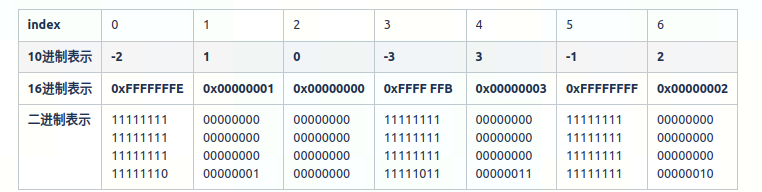
\includegraphics[scale = 0.7]{data0_int32.png}
    \caption{整型输入数据示意图}
    \label{fig:data0_int32}
    % \note{注:图注的内容不宜放到图题中。}
\end{figure}


原始数据经过基数排序后为data1,其表示见下图~\ref{fig:data1_int32}::

\begin{figure}[ht]
    \centering
    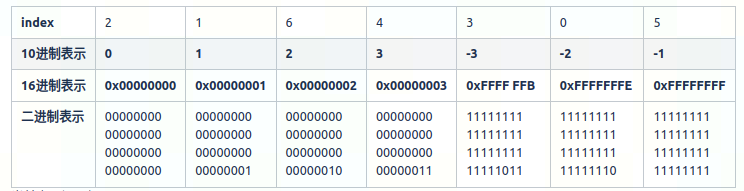
\includegraphics[scale = 0.7]{data1_int32.png}
    \caption{整型数据未处理排序结果示意图}
    \label{fig:data1_int32}
    % \note{注:图注的内容不宜放到图题中。}
\end{figure}


经过基数排序后,结果与预期不符:结果的排布方式为正数为非降序,负数为非降序,且负数在正数后。
对于这种问题目前的解决方案有两种:

a.当升序排序时,预先得到负数和非负数的总个数,
然后据此将正数和负数写回的index进行偏移。
b.对数据进行预处理,对符号位进行变换,在最后再将变换后的数据进行还原。

因为方案b可以直接使用位操作指令,性能更快,且实现更加简便,因此这里使用了方案b进行实现。
具体的实现方案如下:
\begin{description}
\item[预处理]:
因为期望非负数在负数之后,所以直接将所有数的符号位进行取反操作,
即直接将输入数组中的各个元素与0x80000000进行位异或。

\item[后处理]:恢复原来的数据,基数排序完成后index是符合期望的,
现在需要做的是将原始数据revert回来;因此将输出数据再次与0x80000000进行位异或。
\end{description}

上述步骤主要使用到的平台指令为bang\_bxor\_scalar 和 bang\_mlu
即逐个比特位取反, 通过上述处理之后,数据将会正常显示。如图~\ref{fig:res_int32}所示。
\begin{figure}[ht]
    \centering
    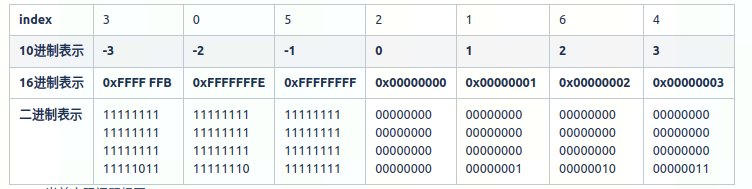
\includegraphics[scale = 0.7]{res_int32.png}
    \caption{整型正确输出示意图}
    \label{fig:res_int32}
    % \note{注:图注的内容不宜放到图题中。}
\end{figure}




(二)浮点数类型

针对浮点数类型数据,基数选择可基于其特定二进制表示形式开展。
在遵循 IEEE 754 标准的浮点数表示中,以float32数据类型为例,
浮点数在内存中的存储分为以下三部分:

符号位(Sign bit):表示浮点数的正负,0 表示正,1 表示负。
指数部分(Exponent):表示浮点数的指数,用偏移量编码(偏移量也称为偏置,为127)。
尾数部分(Mantissa):表示浮点数的有效数字,通常采用归一化表示(即小数点左边默认为 1)。


\begin{figure}[ht]
    \centering
    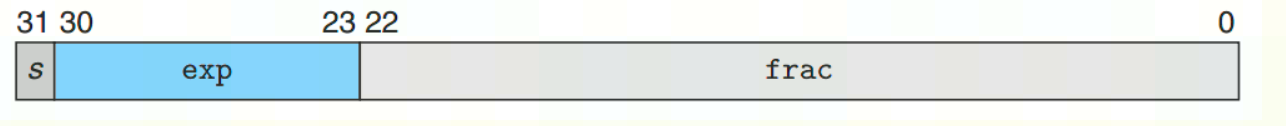
\includegraphics[scale = 0.3]{float32.png}
    \caption{float32数据类型结构图}
    \label{fig:float32}
    % \note{注:图注的内容不宜放到图题中。}
\end{figure}
这种结构设计使得浮点数在数值表示上具有独特的规律,虽然不同于整型数据,但是
其中从 0 到 30 位(除符号位)对数字大小的重要性仍然是依次递增。
同样的,由于符号位的存在,其存在与有符号整数相似的问题(但不完全相同)。
以float数据类型为例,half类型同理。
设原始数据为data0,具体数据为[-2, 1, 0,  -3, 3, -1, 2] 7个float32数据,对其进行
为了更好的说明问题,此处我们同样以基数排序进行问题的说明。

\begin{figure}[ht]
    \centering
    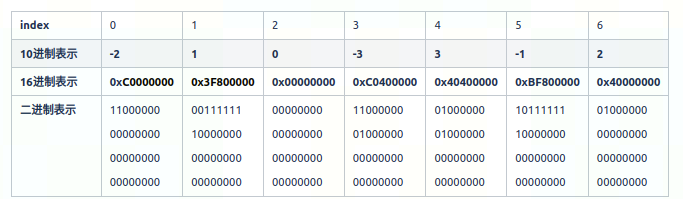
\includegraphics[scale = 0.7]{data0_float32.png}
    \caption{浮点型输入数据示意图}
    \label{fig:data0}
    % \note{注:图注的内容不宜放到图题中。}
\end{figure}


原始数据经过基数排序后的 data1为:

\begin{figure}[ht]
    \centering
    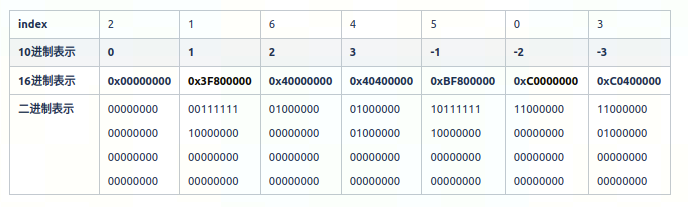
\includegraphics[scale = 0.7]{data1_float32.png}
    \caption{浮点型未处理排序结果示意图}
    \label{fig:data1}
    % \note{注:图注的内容不宜放到图题中。}
\end{figure}


经过基数排序后,结果与预期不符:结果的排布方式为正数为非降序,负数为非升序,且负数在正数后。
对于这种问题目前的解决方案有两种:

a.当升序排序时,预先得到负数和非负数的总个数,
然后据此将正数和负数写回的index进行偏移,同时由于负数为降序排序,
所以将data1中负数内部进行reverse。 

b.对数据进行预处理,对符号位进行变换,在最后再将变换后的数据进行还原。

因为方案b可以直接使用位操作指令,性能更快,且实现更加简便,因此这里使用了方案b进行实现。
具体的实现方案如下:
\begin{description}
\item[预处理]:
因为期望非负数在负数之后,所以考虑将所有数的符号位进行取反操作;
同时期望负数内部为升序排列,所以考虑将负数的非符号位进行取反操作;
即:对正数进行符号位取反,对负数全部bit位进行取反,即非负数数与 0x80000000进行位异或操作, 
负数 与 0xffffffff 进行位异或操作; (任何数与0异或保持不变,与1异或会取反)

\item[后处理]:恢复原来的数据,基数排序完成后index是符合期望的,
现在需要做的是将原始数据revert回来;即将对正数进行符号位取反,
对负数全部bit位进行取反,得到最终结果RES。
\end{description}


通过上述处理之后,数据将会正常显示:

\begin{figure}[ht]
    \centering
    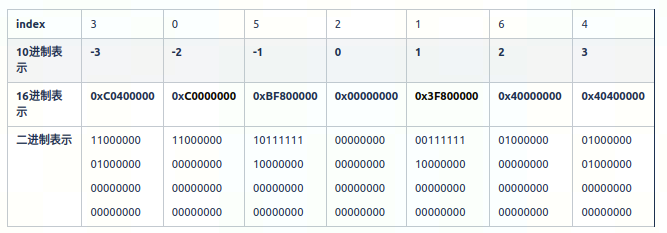
\includegraphics[scale = 0.7]{res_float32.png}
    \caption{整型正确输出示意图}
    \label{fig:res_float32}
    % \note{注:图注的内容不宜放到图题中。}
\end{figure}


上述步骤主要使用到的平台指令及具体作用如下:

a.用来得到区分非负数和负数的mask: bang\_band\_scalar 和 bang\_eq\_scalar

b.按bit取反: bang\_bxor\_scalar 和 bang\_mlu

\subsection{基数选择对最大/最小值的分析}
基于前文针对正负性所展开的讨论,在实施 radix - select 算法的进程中,若预先对数据予以预处理,则 radix - select 函数的功能性能够得到优化,进而无需对数值的正负特性以及数据类型予以过度的关切。鉴于数据预处理所具有的关键意义,本文深入探究了借助数据预处理来达成 radix - select 函数与最大值或最小值相解耦的可行性。通过深入且细致的分析后可知,恰似处理正负性问题的情形,凭借数据预处理的策略,能够将“Top - k 大”的问题有效地转换为“Top - k 小”的问题,从而显著地削减 radix - select 函数在实现过程中的复杂程度。

(一)整数类型
为了更为清晰地阐释相关问题,并且鉴于基数选择算法与基数排序算法之间存在着高度的一致性,下文将以基数排序为例,阐述问题的现象及其对应的解决方案。

设定原始数据为 data0,其具体数据为 [-2, 1, 0, -3, 3, -1, 2] 这 7 个 int32 类型的数据。倘若在此情形下需要获取前 Top - k 大的元素,那么我们能够通过对原数据进行适当的更改,从而将问题转化为“获取前 Top - k 小的元素”。

依据上文的分析,若直接对 data0 执行基数排序操作,将会得到 [0, 1, 2, 3, -3, -2, -1] 这样的排序结果。考虑到我们实际所期望的结果是降序输出,就负数与正数的整体相对位置而言,其输出结果是与预期相符的,故而数据的符号位无需进行变更。然而,针对负数内部的排序结果以及正数内部的排序结果来讲,均与预期的降序结果相互背离。因此,需要对所有数据的非符号位实施取反操作。通过上述一系列的操作处理,我们能够简洁高效地将原始问题进行转换。

(二)浮点数类型
为了更为有效地说明问题,鉴于基数选择算法与基数排序算法之间的紧密关联性,以下将以基数排序作为示例,用以说明问题的现象及其对应的解决方案。

设定原始数据为 data0,其具体数据为 [-2.0, 1.0, 0.0, -3.0, 3.0, -1.0, 2.0] 这 7 个 float32 类型的数据。若在当前情形下需要获取前 Top - k 大的元素,那么我们可通过对原数据进行调整,将问题转化为“获取前 Top - k 小的元素”。

依据前文的分析,若直接对 data0 执行基数排序,将会得到 [0.0, 1.0, 2.0, 3.0, -1.0, -2.0, -3.0] 这样的结果。考虑到我们所需求的结果是降序输出,对于负数而言,无论是负数内部的排序结果,还是负数相对于正数的排序结果,均与预期相契合,因此数据的符号位保持不变且负数无需进行任何改动。而对于非负数部分,由于所期望的输出应当是数值越大其相对顺序越小,所以需要对非负数的非符号位进行取反操作。通过上述的操作流程,我们能够便捷地将原始问题予以转换。 



\section{本章小结}
本章首先概述了国产AI处理器Top-k算子的计算流程,对主要工作进行介绍。随后详细介绍了主机端应该进行的
主要任务,这些任务包括:参数准确性检查,核函数配置,输入预处理和输出后处理。最后详细介绍了设备端
基于RadixSelect算法的并行实现:首先作出了小k/大k场景的划分,而后基于MLU-Core的片上资源分别进行了并行设计与实现。